\documentclass[11pt,a4paper]{article}

\usepackage{pifont}
\usepackage{amsmath}
\usepackage{psfig}
\usepackage{graphicx}
\usepackage{array}
\usepackage{fancyheadings}
\usepackage{here}
\usepackage{eepic,epic}
\usepackage[english]{babel}

\oddsidemargin 0cm
\evensidemargin 0cm
\textwidth 15.5 cm
\topmargin 0cm
\textheight 22cm
\parskip=2mm

\begin{document}


\begin{center}
{\LARGE Extended PDE TOOLBOX Project: \\[0.2cm]
a MATLAB toolbox for Finite Element Methods} \\[0.2cm]
{\large Supported by the Department of Mathematics and Modeling \\[0.2cm]
Institut National des Sciences Appliqu\'ees de Toulouse (INSA) }\\[1.5cm]
\end{center}

\section{Presentation}

The aim of the project is to build a \textsc{matlab} environment for the
approximation of problems modelized with partial differential equations
(PDE's), based on finite element methods (FEM). The implementation will 
take the form of a \textsc{matlab} toolbox, linked to the already existing 
PDE toolbox. It will allow to compute approximate solutions of
various problems (structural mechanics, Stokes problem, heat equation,
Maxwell equations, flow in porous media, ...), and will offer a large set of
different methods (finite elements of arbitrary degree, mixed methods,
finite volume methods, access to basic tools for the approximation of
general problems).

At least at the beginning, this tool will not offer specific tools for
generating meshes, and will rely for this on the existing PDE toolbox of 
\textsc{matlab}. However, even in that context, 3D extensions will be
proposed for some applications. These possibilities should be improved if in
future versions \textsc{matlab} is updated to deal with 3D meshes. 

The project will be based on the following elements.
\begin{itemize}
\item  Knowledge in approximation of PDE problems and finite element methods
at the department and at the MIP laboratory (Math\'{e}matiques pour
l'Industrie et la Physique).

\item  An already existing code \textsc{Getfem++}  (GEneric Tool for Finite
Element Method) which carries out basic computations.

\item  Motivation of the students of the department to work on an
interesting project mixing PDE approximation, real engineering work and
quality requirement.
\end{itemize}

An important effort will be done to exploit graphical possibilities of 
\textsc{matlab} for representing the solutions to PDE problems. The solution
of linear and non-linear system of equations will involve \textsc{matlab}
methods.

The main originality of this project, compared to existent tools, is the
high level of genericity brought by Getfem++. This code allows the
description of  a very large set of finite element methods with the same
formalism \ and arbitrary dimension or degree. Moreover, careful attention
has been given to performance in terms of computational time while building
this code. This genericity allows a fast construction of efficient methods
for a large class of problems. 

There will be two levels for using this toolbox: low-level tools and
high-level tools. Low-level tools will allow to access to the details of the
mesh structure, to the parameterization of the different finite element
methods and  to the computation of arbitrary elementary matrices. This level
should allow a person which is familiar with finite element methods to build
his own approximation, including non-classical PDE problems. This will be a
support for research or pedagogical projects.

The high-level tools will give an easy to use tool for solving problems with
classical methods, including visualization of the solution. Particularly,
the following problems which are not included in the PDE Toolbox will be
available.
\begin{itemize}
\item  fluid mechanics (Stokes, Navier Stokes),

\item  elastic incompressible materials,

\item  dynamical hyperbolic problems using finite volume schemes,

\item  Method of moments (boundary element methods) for 2D and 3D time harmonic Maxwell equations.
\end{itemize}

\section{Context}

The Department of Mathematics and Modeling of INSA Toulouse is a structure
with about 50 researchers, teachers and PhD students, working on Applied
Mathematics. Many of them belong to the MIP laboratory (Math\'{e}matiques
pour l'Industrie et la Physique) which associates Paul SABATIER University,
Toulouse I University, CNRS and INSA. Topics of the MIP laboratory are
scientific computing, optimization, PDE theory, modeling and numerical
analysis (see http://mip.ups-tlse.fr) 

An important support can be expected from the following persons, which are
specialists in their domains.
\begin{itemize}
\item  Abderhamane BENDALI, MIP-INSA: Maxwell equations, finite element
methods, mixed methods, structural mechanics. 

\item  Jean-Paul VILA, MIP-INSA: hyperbolic equations, fluid mechanics,
finite volume methods, flow in porous media. 

\item  Faker BEN BELGACEM, MIP-UPS: Finite element methods, Mortar methods,
mixed methods. 

\item  Philippe GUILLAUME, MIP-INSA: Shape optimization, topological
optimization, 

\item  Patrick LABORDE, MIP-UPS: Structural mechanics, non-linear and
multi-valued constitutive laws, contact and friction,

\item  Yves RENARD, MIP-INSA: Structural mechanics, contact, friction.%
\end{itemize}

The Department of Mathematics and Modeling trains each year around 42
students in Applied Mathematics. About half of them are specialized in
approximation of PDE's. The main part of the programming in the project will
be supported by students work. It is an opportunity to motivate them with a
real size project, underlying re-usability of code, documentation, strict
rules of programming and project management. 

This toolbox will provide interesting tools in several research projects of
the laboratory MIP. This  will be helpful to test and improve the efficiency
of the toolbox. 

\section{Already existing code Getfem++}

The code \textsc{Getfem++} (GEneric Tool for Finite Element Methods) is a
C++ library based on an object and iterator oriented programming, which
makes it a performing and generic tool for finite element methods. This
library has been developed by Yves RENARD at the Department of Mathematics
and is already used for applications such as friction problems in structural 
mechanics and diphasic flow in porous media. 

The main features of this library can be summarized as follows.
\begin{itemize}
\item  mesh management. A mesh structure which is able to store and modify a
set of elements with arbitrary shape and arbitrary dimension. Basic elements
are the simplexes (segments, triangles, tetrahedrons,... ) and direct
product of simplexes (quadrilaterals, prisms,...). A particular mesh can
contain elements of different dimensions.

\item  A description of finite element methods which is separated into the
description of
\begin{itemize}
\item  geometric transformations (linear for basic elements,  non-linear for
example for iso-parametric elements),

\item  approximated or exact integration methods,

\item  interpolation methods (nodes and shape functions).
\end{itemize}

A FEM is defined by these three elements. In particular, $P_{K}$
finite elements on simplexes of arbitrary dimension are defined ($K\geq 0$
is the degree of the polynomials), as well as tensor product of $P_{K}$
elements on quadrilaterals or prisms.

\item  Description and computation of elementary matrices. The proposed
description of element matrices allows to compute all types of element
matrices needed for the approximation of standard problems, including mixed
methods.

\item  Assembling systems for classical problems (Stokes, linear elasticity,
... ) and classical boundary conditions.
\end{itemize}

\begin{figure}[htbp]
\begin{center}
\begin{tabular}{ccc}
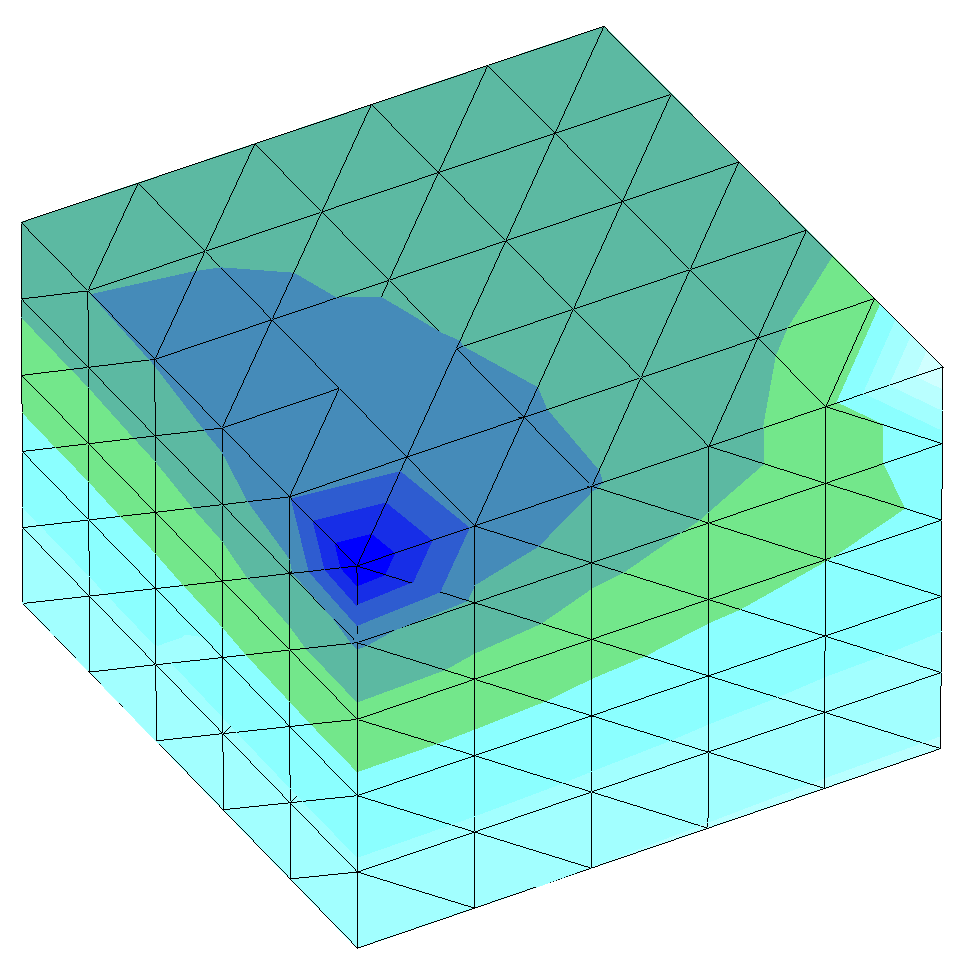
\includegraphics[width=7cm,angle=0]{getfem_presentation_press.eps} & \hspace{1em} & %
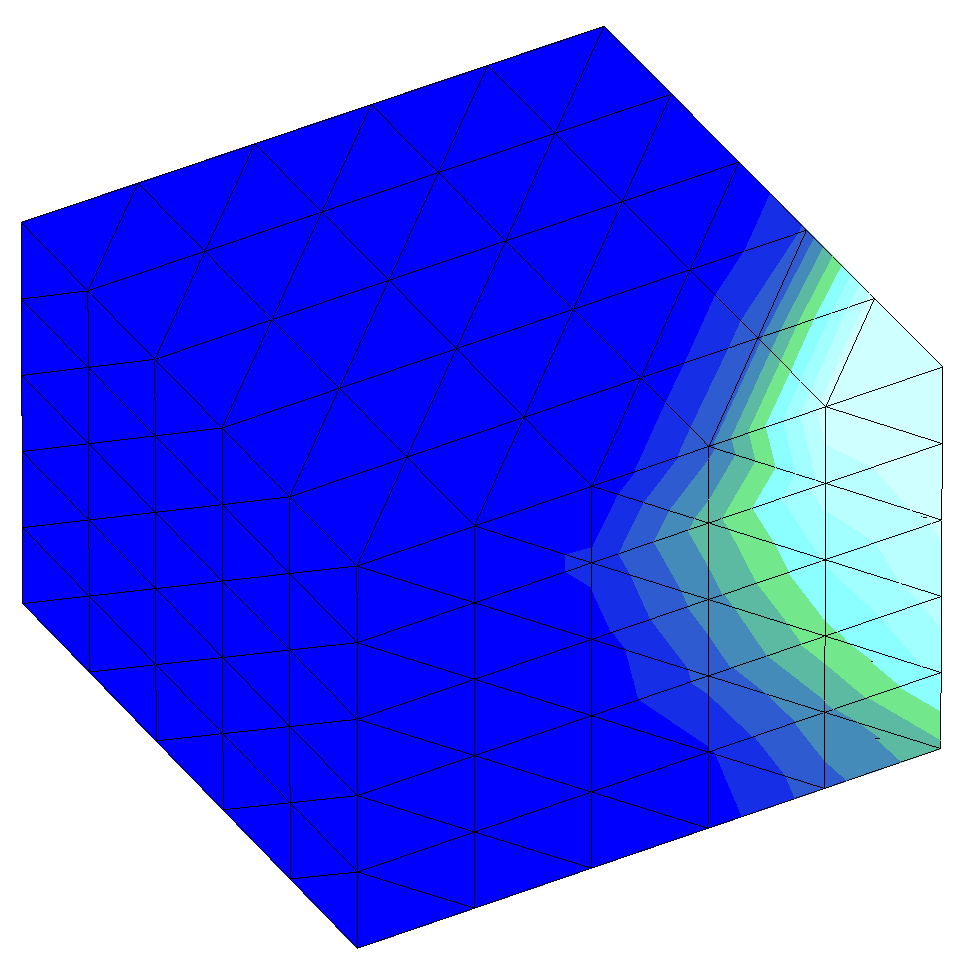
\includegraphics[width=7cm,angle=0]{getfem_presentation_sat.eps} \\ 
pressure &  & saturation
\end{tabular}
\end{center}
\caption{\textit{Example of computation using getfem++ for a diphasic flow
in porous media. }}
\label{fig:body}
\end{figure}

\section{Short term objective}

For the first step, the objective is to provide a finalized and coherent
toolbox with the following features.
\begin{itemize}
\item  a \textsc{matlab} interface to perform basic computations with 
\textsc{Getfem++}  accessible in the \textsc{matlab} environment. This
allows the possibility accessing to the mesh structure, modifying it,
accessing to each element, defining a particular finite element method on
each element of the mesh, accessing to finite element nodes, to the global
numbering of the nodes, and the possibility defining and computing any
element matrix on an element or on a face of an element.

\item  Input and Output based on the PDE toolbox with functions similar to
``assempde'' (possibly with the same syntax) but with larger possibilities ($%
P_{K}$ elements ...), for linearized elasticity, Maxwell equations and heat
equation.

\item  Mixed methods for Stokes problem and for elastic incompressible
materials.
\end{itemize}

3D problems (and even 4D, for a full-Galerkin approach) will be supported
(with some methods to import meshes) but not fully interfaced (methods will
be given to transform a 2D mesh in a 3D prismatic or tetrahedric mesh).

\section{Medium term objective}

Once this base is constructed, a strong motivation should exist to develop
extensions on various domain, such as
\begin{itemize}
\item  additional finite elements:
\begin{itemize}
\item  high degree iso-parametric elements (for structural mechanics),

\item  Hermite elements (for plate problems),
\end{itemize}

\item  additional classical problems:
\begin{itemize}
\item  Navier Stokes equation,

\item  contact problems in linear elasticity,

\item  hyper-elasticity (large deformation elasticity),

\item  flow in porous media,

\item  plates problems,

\item  3D Maxwell problem,
\end{itemize}

\item  Extended graphical visualization,

\item  Graphical interfaces for some problems.
\end{itemize}

\end{document}




